\chapter{Validaci\'on y Resultados}
\label{chap:resultados}

%\endinput

\section{Introducci\'on}
En este cap\'itulo presentamos los distintos escenarios que fueron planteados para la validaci\'on de los procesos.\\
Dado que para la metodolog\'ia de estimaci\'on de errores que proponemos utilizamos datos reales de una misi\'on operativa argentina, hubiera sido
deseable contar con datos de alertas de colisiones reales propias de esa misi\'on, ya que esto nos hubiera permitido hacer una validaci\'on end-to-end de todo el prototipo. No obstante, por cuestiones de confidencialidad y pol\'iticas que fueron modific\'andose, no fue posible tener acceso a esa informaci\'on, que seg\'un nos comunicaron, fue borrada una vez finalizada la misi\'on.\\
Frente a este panorama, presentamos a continuaci\'on la secuencia de etapas de validaci\'on que permiten evaluar, cada una de las etapas del procesamiento.\\

En primer lugar fue fundamental corroborar las propagaciones de los TLEs realizadas con la librer\'ia de python {\it{sgp4-1}} \citep{sgp4python}, para ello utilizamos la versi\'on de prueba que ofrece el software STK (System Tool Kit) \citep{stk}.\\
Para la validaci\'on de los resultados de la implementaci\'on del m\'etodo de Osweiler en la generaci\'on de matrices de covarianza, comparamos nuestros resultados para los distintos escenarios que se publican en el trabajo.\\

El m\'etodo que proponemos para la estimaci\'on de la propagaci\'on de errores, es el que m\'as dificultades present\'o para ser validado. Ya que al basarse plenamente en los datos de la misi\'on cuyos resultados de colisi\'on de alerta no nos fueron suministrados, fue analizado en comparaci\'on con resultados estad\'isticos globales, o sobre el estudio de encuentros de otras misiones y esto implica una variaci\'on en si mismo.\\

Finalmente la implementaci\'on del c\'alculo de probabilidad de colisi\'on fue evaluado a partir de la recopilaci\'on de bibliograf\'ia con datos de encuentros anteriores.\\

\section{Implentenaci\'on del modelo SGP4 en Python}

Para la propagaci\'on de las posiciones orbitales con el modelo SGP4 (Sec. \ref{subsec:sgp4model}) utilizamos la librer\'ia de python {\bf{sgp4-1}} \citep{sgp4python}.
Luego usamos el software {\it{Systems Tool Kit (STK)}} \citep{stk} para comparar nuestras propagaciones y asegurarnos la correcta utilizaci\'on y configuraci\'on de la librer\'ia sgp4-1.\\

Se listan a continuaci\'on dos tablas con las efem\'erides de la misi\'on, correspondientes a los primeros cuatro minutos del d\'ia 01/01/2013.
Ambas fueron generadas a partir del mismo TLE y presentas resultados que difieren en algunos metros para los peores casos. Resultado aceptable, teniendo en cuenta que las estimaciones groseras de errores para las propagaciones hechas con TLEs y SGP4 acarrean errores de kil\'ometros o decenas de kil\'ometros.\\

\underline{TLE.}
{\small
\begin{verbatim}
1 xxxxU xxxxx   13001.74853505  .00000428  00000-0  75550-4 0  9996
2 xxxxx 098.0122 011.5654 0001526 107.5603 009.0604 14.72289948 84036
\end{verbatim}}


\begin{table}[!h]
\centering
\resizebox{14cm}{!}{
\begin{tabular}{lcccccc}
Epoca & x [km] & y [km] & z [km] & vx $[km/s]$ & vy $[km/s]$ & vz $[km/s]$\\
\hline
2013-01-01 00:00&-2372.76245& -1381.01830& 6465.57494& -6.95099& -0.93631& -2.74523\\
2013-01-01 00:01& -2784.64672& -1434.31269& 6287.6158& -6.77374& -0.83955& -3.18470\\
2013-01-01 00:02& -3185.05363& -1481.69530& 6083.67196& -6.56854& -0.73932& -3.61109\\
2013-01-01 00:03& -3572.3305& -1522.96975& 5854.58154& -6.336229& -0.63602& -4.02263\\
2013-01-01 00:04& -3944.8780& -1557.96472& 5601.28702& -6.077737& -0.53007& -4.417616\\
\hline
\label{tab:arcode}
\end{tabular}
}
\caption{Resultados que genera ARxCODE utilizando la librer\'ia sgp4 de python para la propagaci\'on.}
\end{table}

\begin{table}[!h]
\centering
\resizebox{14cm}{!}{
\begin{tabular}{lcccccc}
% \hline
\'Epoca & x [km] & y [km] & z [km] & vx [km/s] & vy [km/s] & vz [km/s]\\
\hline
2013-01-01 00:00&-2372.76302&-1381.02018&6465.57433&-6.95099&-0.93631&-2.74523\\
2013-01-01 00:01&-2784.64726&-1434.31473&6287.61518&-6.77374&-0.83955&-3.18470\\
2013-01-01 00:02&-3185.05413&-1481.69750&6083.67116&-6.56854&-0.73932&-3.61109\\
2013-01-01 00:03&-3572.33097&-1522.97210&5854.58064&-6.33622&-0.63602&-4.02263\\
2013-01-01 00:04&-3944.87849&-1557.96721&5601.28604&-6.07773&-0.53008&-4.41761
\label{tab:stk}
\end{tabular}
}
\caption{Resultados del Systems Tool Kit (STK) propagando el mismo TLE que ARxCODE.}
\end{table}


\textcolor{red}{hacer las diferencias en python y publicarlas}

\section{Estudio de errores de TLE con datos hist\'oricos}

El trabajo de Osweiler publica los resultados de las matrices de covarianza generadas, para 6 misiones y 8 ventanas de tiempo.\\
Para la validaci\'on se tomaron dos escenarios muy diferentes en cuanto a la altura del sat\'elite: LAGEOS-1 a m\'as de $5000 km$ y ICESAT a $600 km$
Se presentan a continuaci\'on las tablas con los resultados comparativos, entre los valores publicados y los valores obtenidos por ARxCODE.\\
Puede apreciarse, que los errores son muy grandes para el ICESAT, de baja altura, que se ve m\'as perturbado por el efecto atmosf\'erico, que no es modelable con precisión; mientras que el LAGEOS-1 presenta errores muchos \'ordenes de magnitud menor.\\

\begin{table}
 \centering
      \begin{tabular}{cccccc}
      \hline
      Nombre & ID NORAD & Altura & Ecc. & Inclinaci\'on & B* \\
      \hline
      LAGEOS-1 & 8820 & $5850$ & $0.004$ & $109.8$ & $0.0001$ \\
      ICESAT & 27642 & $600$ & $0.0002 - 0.001$ & $94$ & var\'ia \\
      \hline
      \end{tabular}
    \caption[Sat\'elites de Estudio]{Resumen de las caracter\'isticas de los sat\'elites a analizar}
\end{table}

\subsection*{Tablas comparativas ICESAT}

\begin{table}[!h]
\centering
\makebox[0pt][c]{\parbox{1.0\textwidth}{%
    \begin{minipage}[t]{0.48\hsize}\centering
     \resizebox{8cm}{!}{
    \begin{tabular}{cccc}
      \hline
    Vent 1 & $R_{v}$ (km) & $R_{n}$ (km) & $R_{c}$ (km)\\
    \hline
    $R_{v}$ &  2667.377375  &    27.248658   &   -8.22221222\\
    $R_{n}$ & 27.248658  &   0.34323269 & -0.12314379\\
    $R_{c}$ & -8.22221222 & -0.12314379 & 0.07316443\\
    \hline
    \end{tabular}}
      \caption{Matriz de Covarianza de la Bilbiografia \citep{Osweiler} - Sat\'elite ICESAT en la ventana temporal del 1-Mar-03 al 16-Mar-03}
      \label{tab:singlebest}
    \end{minipage}
    \begin{minipage}[t]{0.48\hsize}\centering
    \resizebox{8cm}{!}{
      \begin{tabular}{cccc}
	\hline
      Vent 1 & $R_{v}$ (km) & $R_{n}$ (km) & $R_{c}$ (km)\\
      \hline
      $R_{v}$ &  2667.37364259 &   27.2488814  &   -8.22232626\\
      $R_{n}$ & 27.2488814  &  0.3432413 &  -0.12314867\\
      $R_{c}$ & -8.22232626 & -0.12314867 &  0.073167\\
      \hline
      \end{tabular}}
        \caption{Matriz de Covarianza que produce ARxCODE - Sat\'elite ICESAT en la ventana temporal del 1-Mar-03 al 16-Mar-03}
        \label{tab:twobest}
    \end{minipage}
    \hfill
}}
\end{table}

\begin{table}[!h]
\centering
 \begin{tabular}{cccc}
  \hline
 Vent 1 & Dif.$R_{v}$ (km) & Dif.$R_{n}$ (km) & Dif.$R_{c}$ (km)\\
 \hline
 Dif. $R_{v}$ & -0.00373241 & 0.0002234 & -0.00011404 \\
 Dif. $R_{n}$ &  0.0002234 &  0.000008 & -0.000004\\
 Dif. $R_{c}$ & -0.00011404  & -0.000004 &  0.000002\\
 \hline
 \end{tabular}
 \caption{Diferencias de los valores calculados por ARxCODE respecto a los valores publicados en el trabajo de Osweiler \citep{Oseweiler}}
\end{table}


\subsection*{Tablas comparativas LAGEOS-1}


\begin{table}[!h]
\centering
\makebox[0pt][c]{\parbox{1.0\textwidth}{%
    \begin{minipage}[b]{0.48\hsize}\centering
     \resizebox{8cm}{!}{
    \begin{tabular}{cccc}
      \hline
    Vent 1 & $R_{v}$ (km) & $R_{n}$ (km) & $R_{c}$ (km)\\
    \hline
    $R_{v}$ & 0.378619 & -0.0343598 & 0.02771527 \\
    $R_{n}$ & -0.0343598 &  0.004002 & -0.0027171 \\
    $R_{c}$ & 0.02771527 & -0.0027171 &  0.0084302 \\
    \hline
    \end{tabular}}
      \caption{Matriz de Covarianza de la Bilbiografia \citep{Osweiler} - Sat\'elite LAGEOS-1 en la ventana temporal del 1-Mar-03 al 16-Mar-03}
      \label{tab:singlebest}
    \end{minipage}
    \hfill
    \begin{minipage}[b]{0.48\hsize}\centering
    \resizebox{8cm}{!}{
      \begin{tabular}{cccc}
	\hline
      Vent 1 & $R_{v}$ (km) & $R_{n}$ (km) & $R_{c}$ (km)\\
      \hline
      $R_{v}$ &  0.37863904 & -0.03440871 & 0.02772177 \\
      $R_{n}$ & -0.03440871 & 0.00401173 & -0.00272334 \\
      $R_{c}$ & 0.02772177 & -0.00272334 & 0.00843443\\
      \hline
      \end{tabular}}
        \caption{Matriz de Covarianza que produce ARxCODE - Sat\'elite LAGEOS-1 en la ventana temporal del 1-Mar-03 al 16-Mar-03}
        \label{tab:twobest}
    \end{minipage}
    \hfill
}}
\end{table}

\begin{table}[!h]
\centering
 \begin{tabular}{cccc}
  \hline
 Vent 1 & Dif.$R_{v}$ (km) & Dif.$R_{n}$ (km) & Dif.$R_{c}$ (km)\\
 \hline
 Dif. $R_{v}$ & 0.000020 &  -0.000048 &  0.000006 \\
 Dif. $R_{n}$ & -0.000048 &   0.000009 &  -0.000006 \\
 Dif. $R_{c}$ & 0.000006 &  -0.000006 &   0.000004 \\
 \hline
 \end{tabular}
 \caption{Diferencias de los valores calculados por ARxCODE respecto a los valores publicados en el trabajo de Osweiler \citep{Oseweiler}}
\end{table}

\subsection*{Diferencias de los escenarios todos contra todos}
Estudio hecho sobre los errores que se producen en las propagaciones de los TLE en funci\'on de la cantidad de d\'ias que se propaguen.\\

\begin{figure}[h!]
\centering
  \subfigure[Diferencias ICESAT - ARxCODE]{
    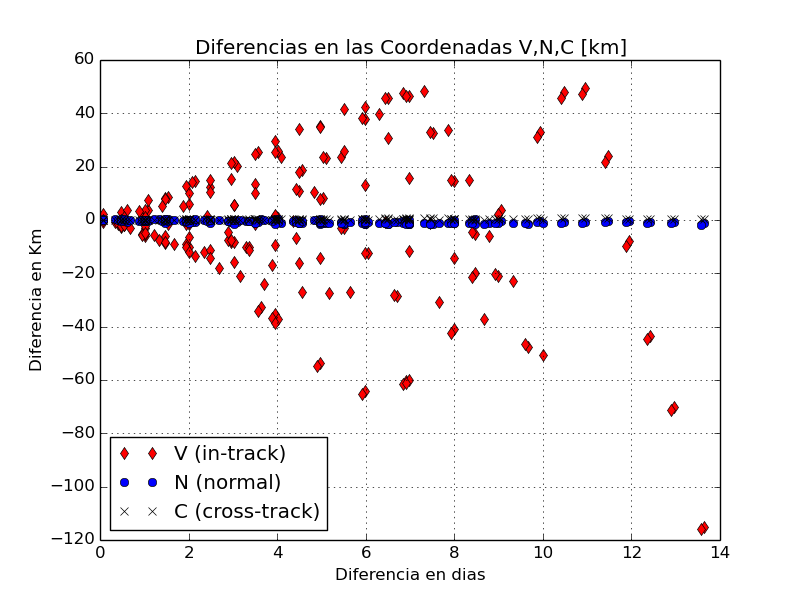
\includegraphics[width=0.48\textwidth]{imagenes/TLEdifTot27642esc52}
  }
  \subfigure[Diferencias ICESAT - Osweiler]{
    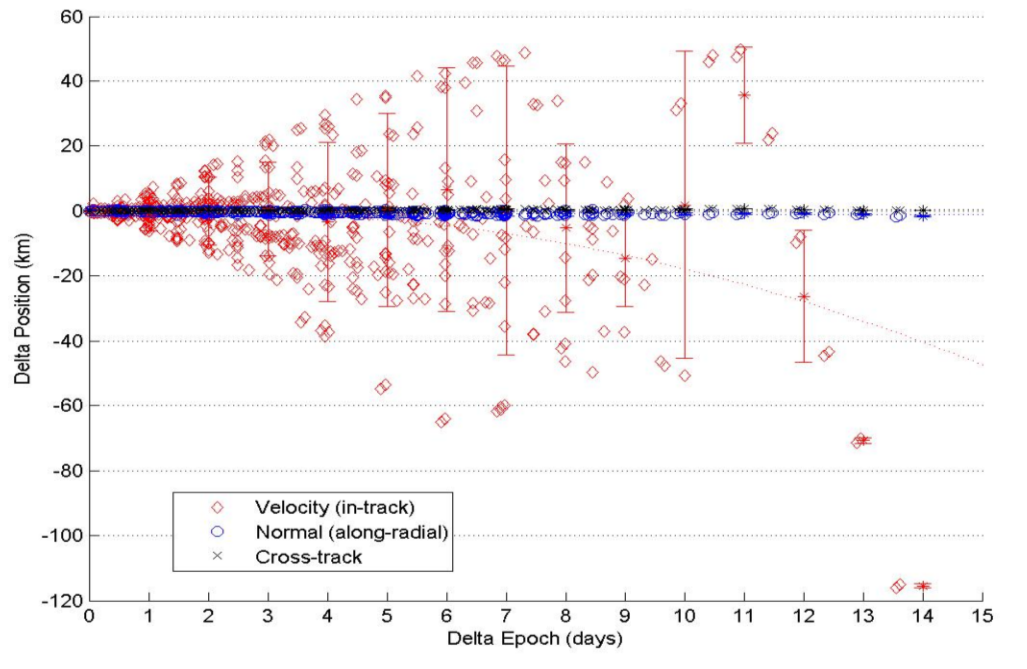
\includegraphics[width=0.48\columnwidth, keepaspectratio]{imagenes/ICESATdifTot}
  }
  \caption{Gr\'afico con Diferencias Totales del escenario ICESAT}
  \label{fig:icesatTot}
\end{figure}

\begin{figure}[h!]
\centering
  \subfigure[Diferencias LAGEOS-1 - ARxCODE]{
    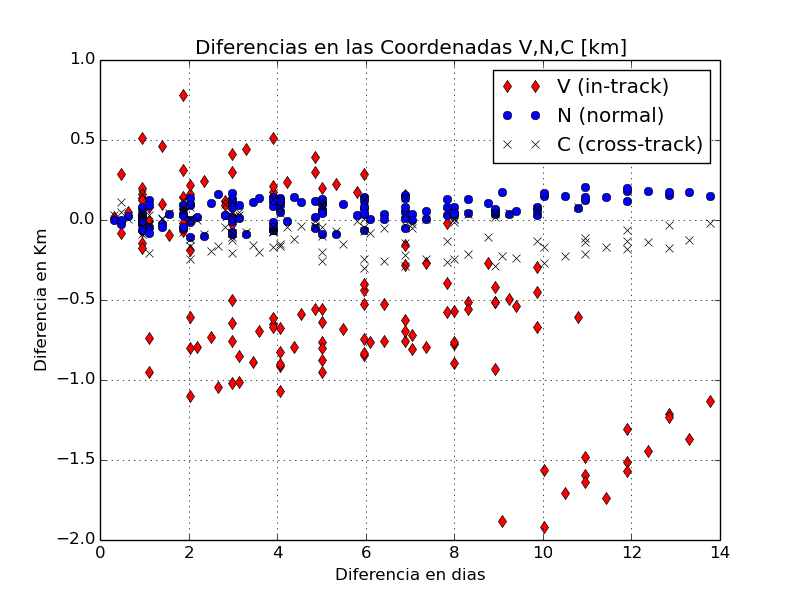
\includegraphics[width=0.48\textwidth]{imagenes/TLEdifTot8820esc11}
  }
  \subfigure[Diferencias LAGEOS-1 - ARxCODE]{
    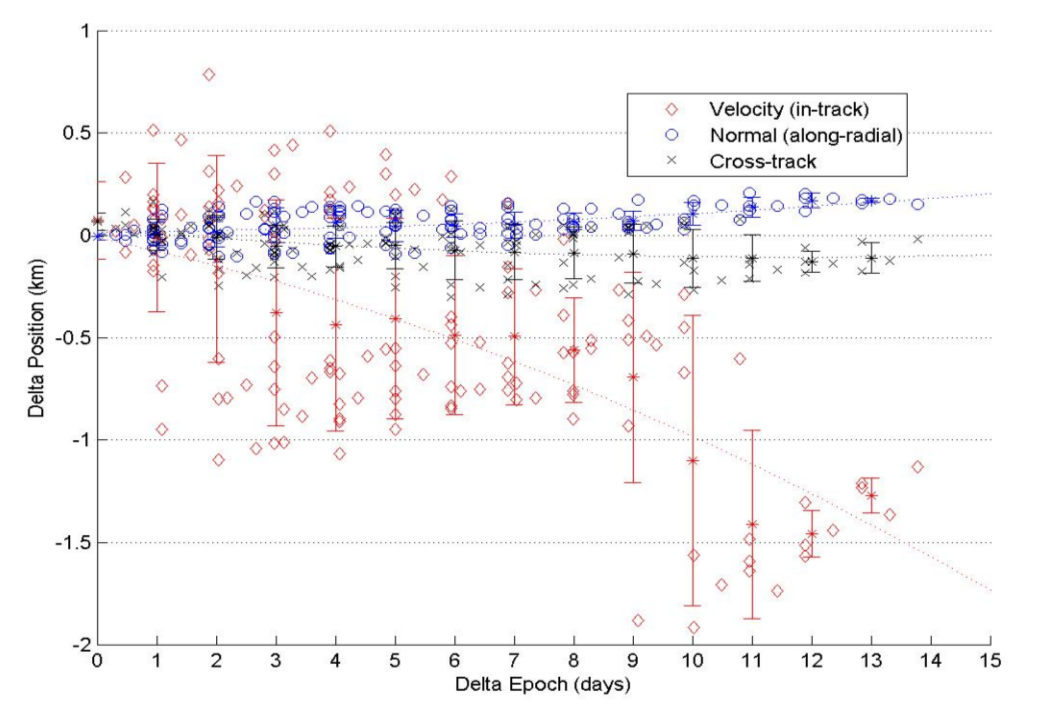
\includegraphics[width=0.48\columnwidth, keepaspectratio]{imagenes/LAGEOSdifTot}
  }
  \caption{Gr\'afico con Diferencias Totales del escenario LAGEOS-1}
  \label{fig:lageosTot}
\end{figure}


\section{Estudio de errores de TLE contra efem\'erides precisas}
\subsection*{Sistema de referencia TOD}
Como ya mencionamos \textcolor{red}{debe haber una secci\'on dedicada a datos CODS}, los productos del departamento de din\'amica orbital con los que trabajamos ofrecen las posiciones orbitales en el sistema de referencia verdadero de la fecha \ac{TOD}, mientras que los resultados de las propagaciones con el sgp4 se encuentran en el sistema \ac{TEME}. Para poder hacer comparaciones desarrollamos un m\'odulo que transforma las coordenadas y velocidades, del sistema TEME al sistema TOD. (Ver. \textcolor{red}{apendice}).
Para la validaci\'on del mismo, utilizamos TLEs de la misi\'on y los propagamos con el sgp4. Los resultados que obtuvimos (en el sistema TEME), los transformamos al sistema TOD con el m\'odulo de transformaci\'on desarrollado y luego lo comparamos con los productos de din\'amica orbital, para los mismos instantes.\\

\textcolor{red}{buscar esos resultados}


\subsection*{Estad\'istica de Errores}
Con la certeza de que los datos eran compatibles y pod\'ian ser comparados, iniciamos el procesamiento de comparaci\'on de las posiciones y la generaci\'on de los resultados estad\'isticos para la propagaci\'on de errores que describimos en la Sec. \ref{sec:properrores}.

En un pre-procesamiento sobre un periodo amplio de la misi\'on, constatamos que fuera de los intervalos de maniobras por commissioning o maniobras de rutina, los TLE presentan un error que es {\it{acotado}}, {\it{estable}} y/o modelable.  

\begin{figure}[!h]
\centering
  \textbf{Tendencia Anual 01/01/2013 - 30/08/2013}\par\medskip
  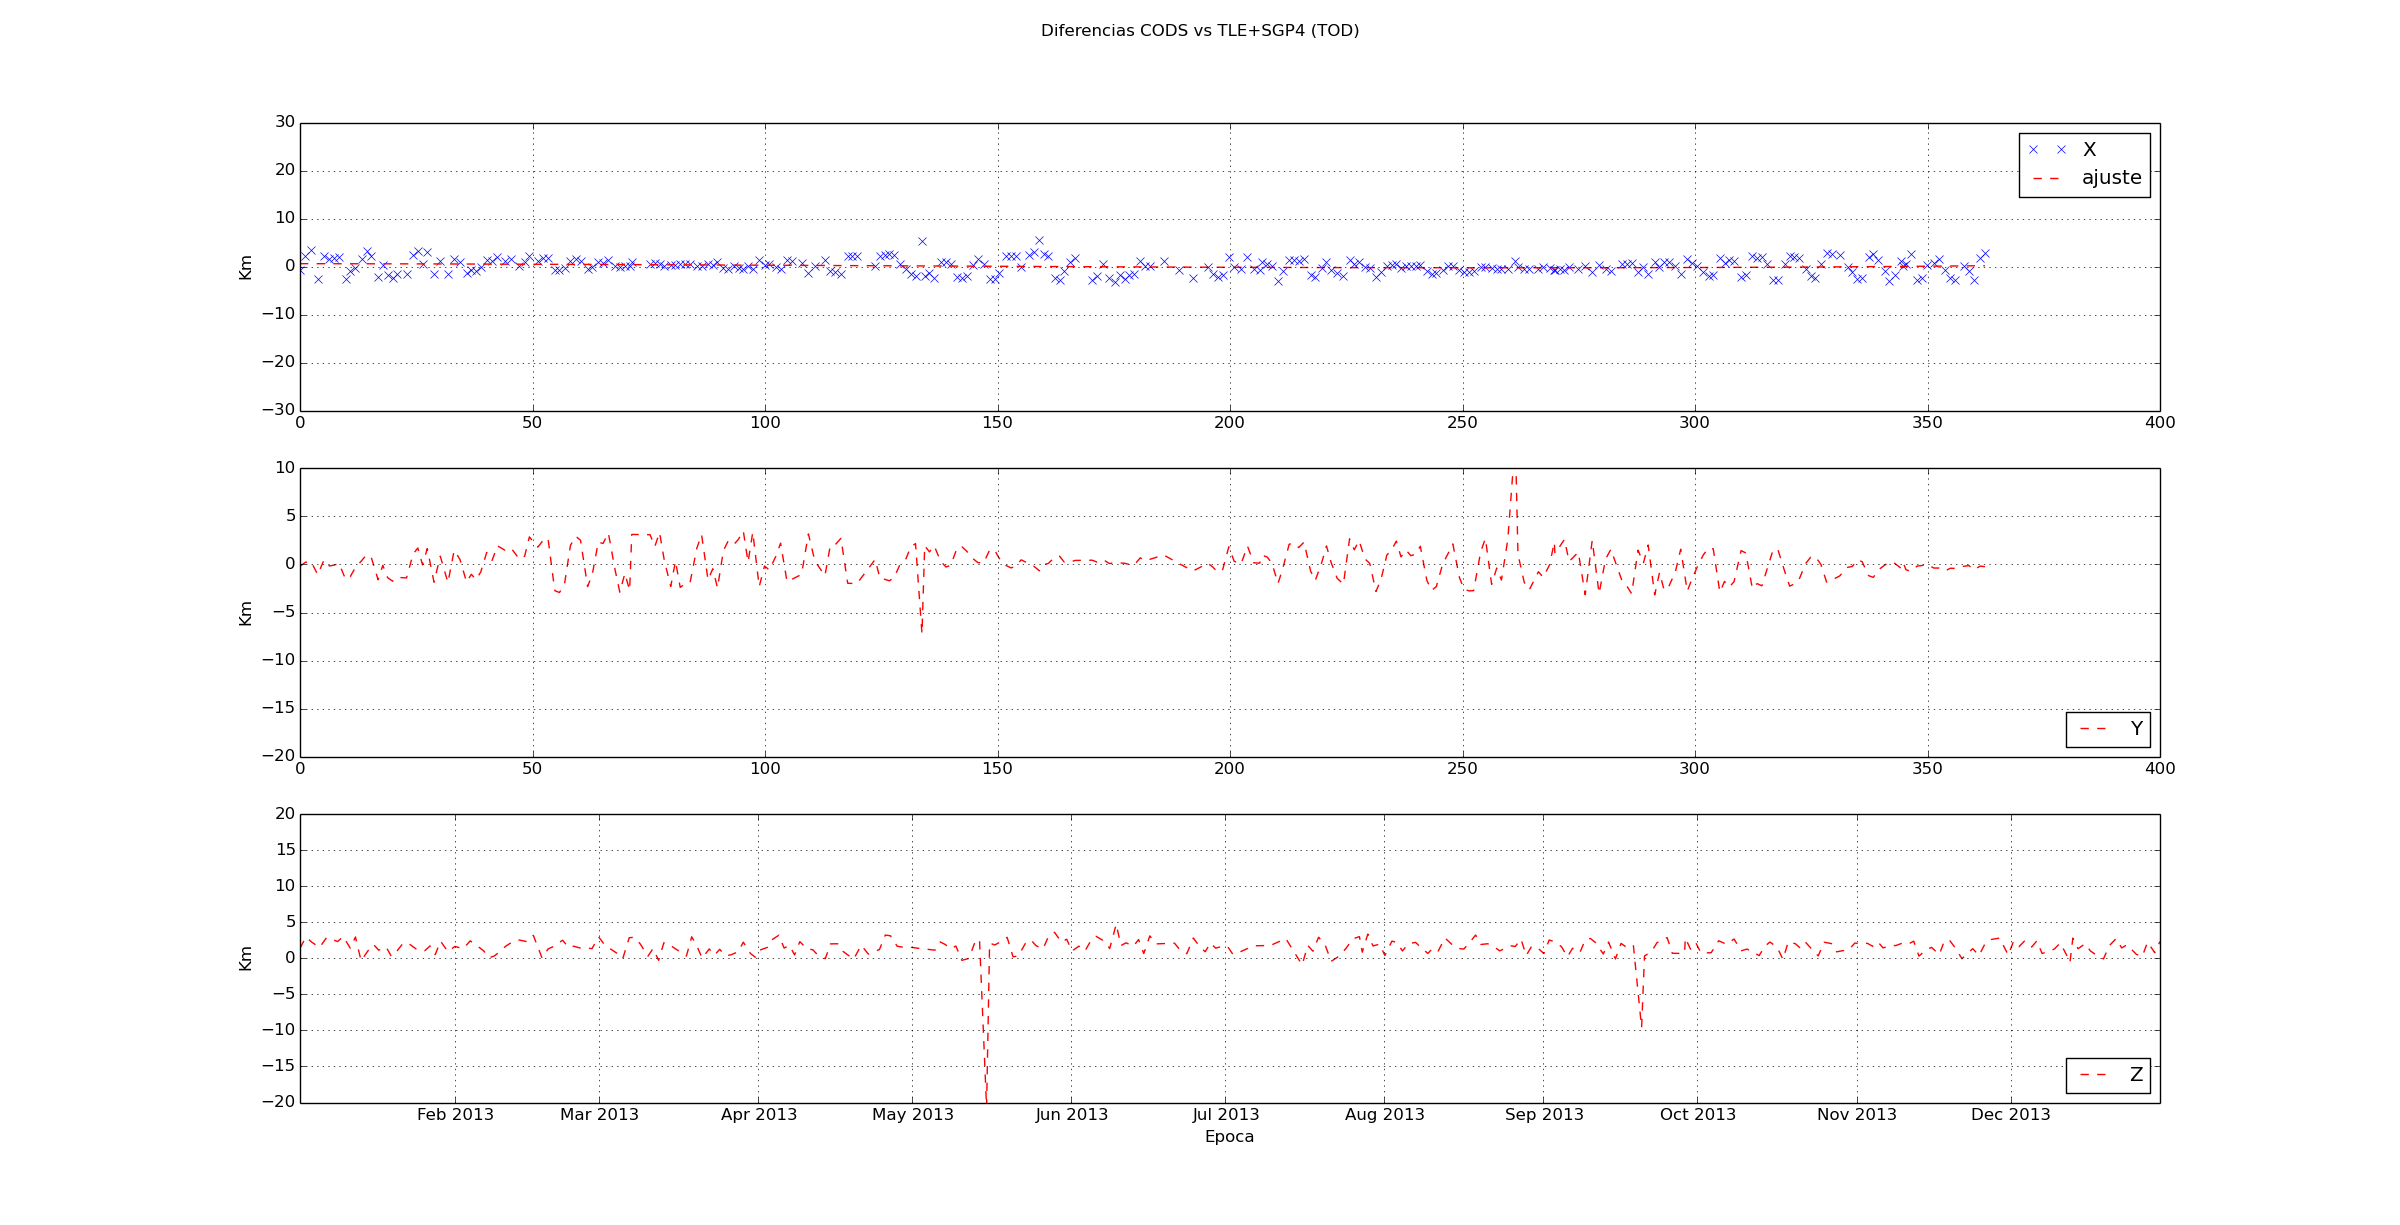
\includegraphics[width=\textwidth]{imagenes/SACD2013todEjesajustados}
  \caption{Tendencia anual de las diferencias contra los datos de din\'amica orbital en coordenadas cartesianas del Sistema TOD}
\end{figure}


% \section{C\'alculo de la Probabilidad de Colisi\'on}
% \begin{figure}[!h]
% \centering
%  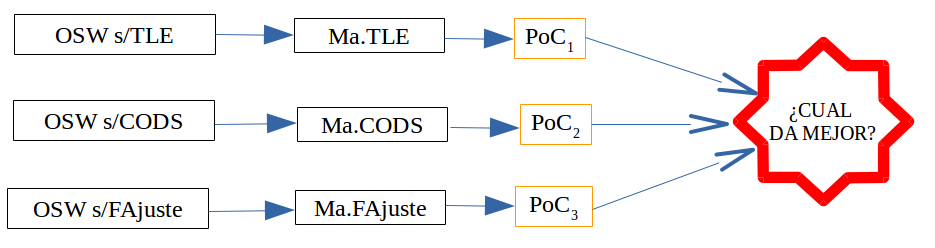
\includegraphics[width=0.5\textwidth]{imagenes/metodoARxCODE}
%  \caption{Metodolog\'ia Propuesta}
%  \label{fig:metodoARxCODE}
% \end{figure}

